\section{Introduction}

As the availability of genetic data has increased,
so has our ability to infer evolutionary processes at finer scales.
An essential tool for evolutionary inference has been simulations,
and many flexible and efficient evolutionary simulators have been developed over the past decade.
Until recently, little had been done to integrate different tools and to ensure compatibility of inferred models across studies.

A unifying thread that has emerged is the use of tree sequence data structure.
The tree sequence provides a way of concisely representing correlated genealogies along chromosomes.
Both msprime, an efficient coalescent simulator, and SLiM, the most widely used forward-in-time simulator,
record the genealogical history of all samples in a population in the form of tree sequences.
One of the major advantages of doing so in forward-in-time simulations is that it allows neutral mutations to be omitted.
By definition, such mutations do not impact the underlying genealogies, but they pose immense computational demand (due to bookkeeping).
Therefore, by omitting the neutral mutations from the forward step, it is possible to decrease computational resources dramatically.
After completion of the forward simulation, it is possible to simply overlay the genealogies with the neutral mutations if necessary.

As inference becomes ever more complex, now enabled by powerful simulation tools,
the need for easy and error-free dissemination of estimated models has increased.
Many researchers used to re-implement models independently,
a process which is error-prone and results in duplication of effort.
Indeed, a recent study described errors in the implementation of a demographic model in two published papers,
which affected the interpretation of biological signals.

Stdpopsim is a community-driven open source developed to minimize these issues.
We organized a well-documented library with published simulation models from a range of organisms,
which can be accessed with simple Python and command-line interfaces.
The library contains demographic models, recombination maps and mutation rates for tens of species.
All the models have to pass a quality control method, in which an independent party validates the model independently.
Further, we provide a Python API to easily run simulations using the catalog, with msprime and SLiM as simulators on the backend,
decreasing even further the barrier to reproducing simulations.

In this chapter, I will present two vignettes of my contributions to the ecosystem of evolutionary simulation tools.
First, I describe a way to parallelize forward-in-time simulations.
Second, I describe the inclusion of selection models to stdpopsim,
and I illustrate the utility of stdpopsim by studying the power to detect sweeps along chromosomes.


\section{Parallelizing forward-in-time simulations}

A major problem in simulation-based inference is the computational cost of simulations.
In many cases, it is possible to minimize the time cost of simulations by running them in parallel,
that is to divide up the simulation over many processes that can be executed concurrently over many CPUs (or cores).
It is not always that it is clear how to divide a simulation into sub-tasks.

In the case of evolutionary simulations, a natural way to break up a big simulation might be population splits.
After a population splits into two (or more) subpopulations, their histories become independent (assuming no migration).
Therefore, it is possible to parallelize a multi-population simulation by dividing the simulation over population splits.
The history of populations A, B and C (shown in \lcref{fig:pop_hist}) can be parallelized:
any two branches stemming from the same node are independent.

\begin{figure}[htp]
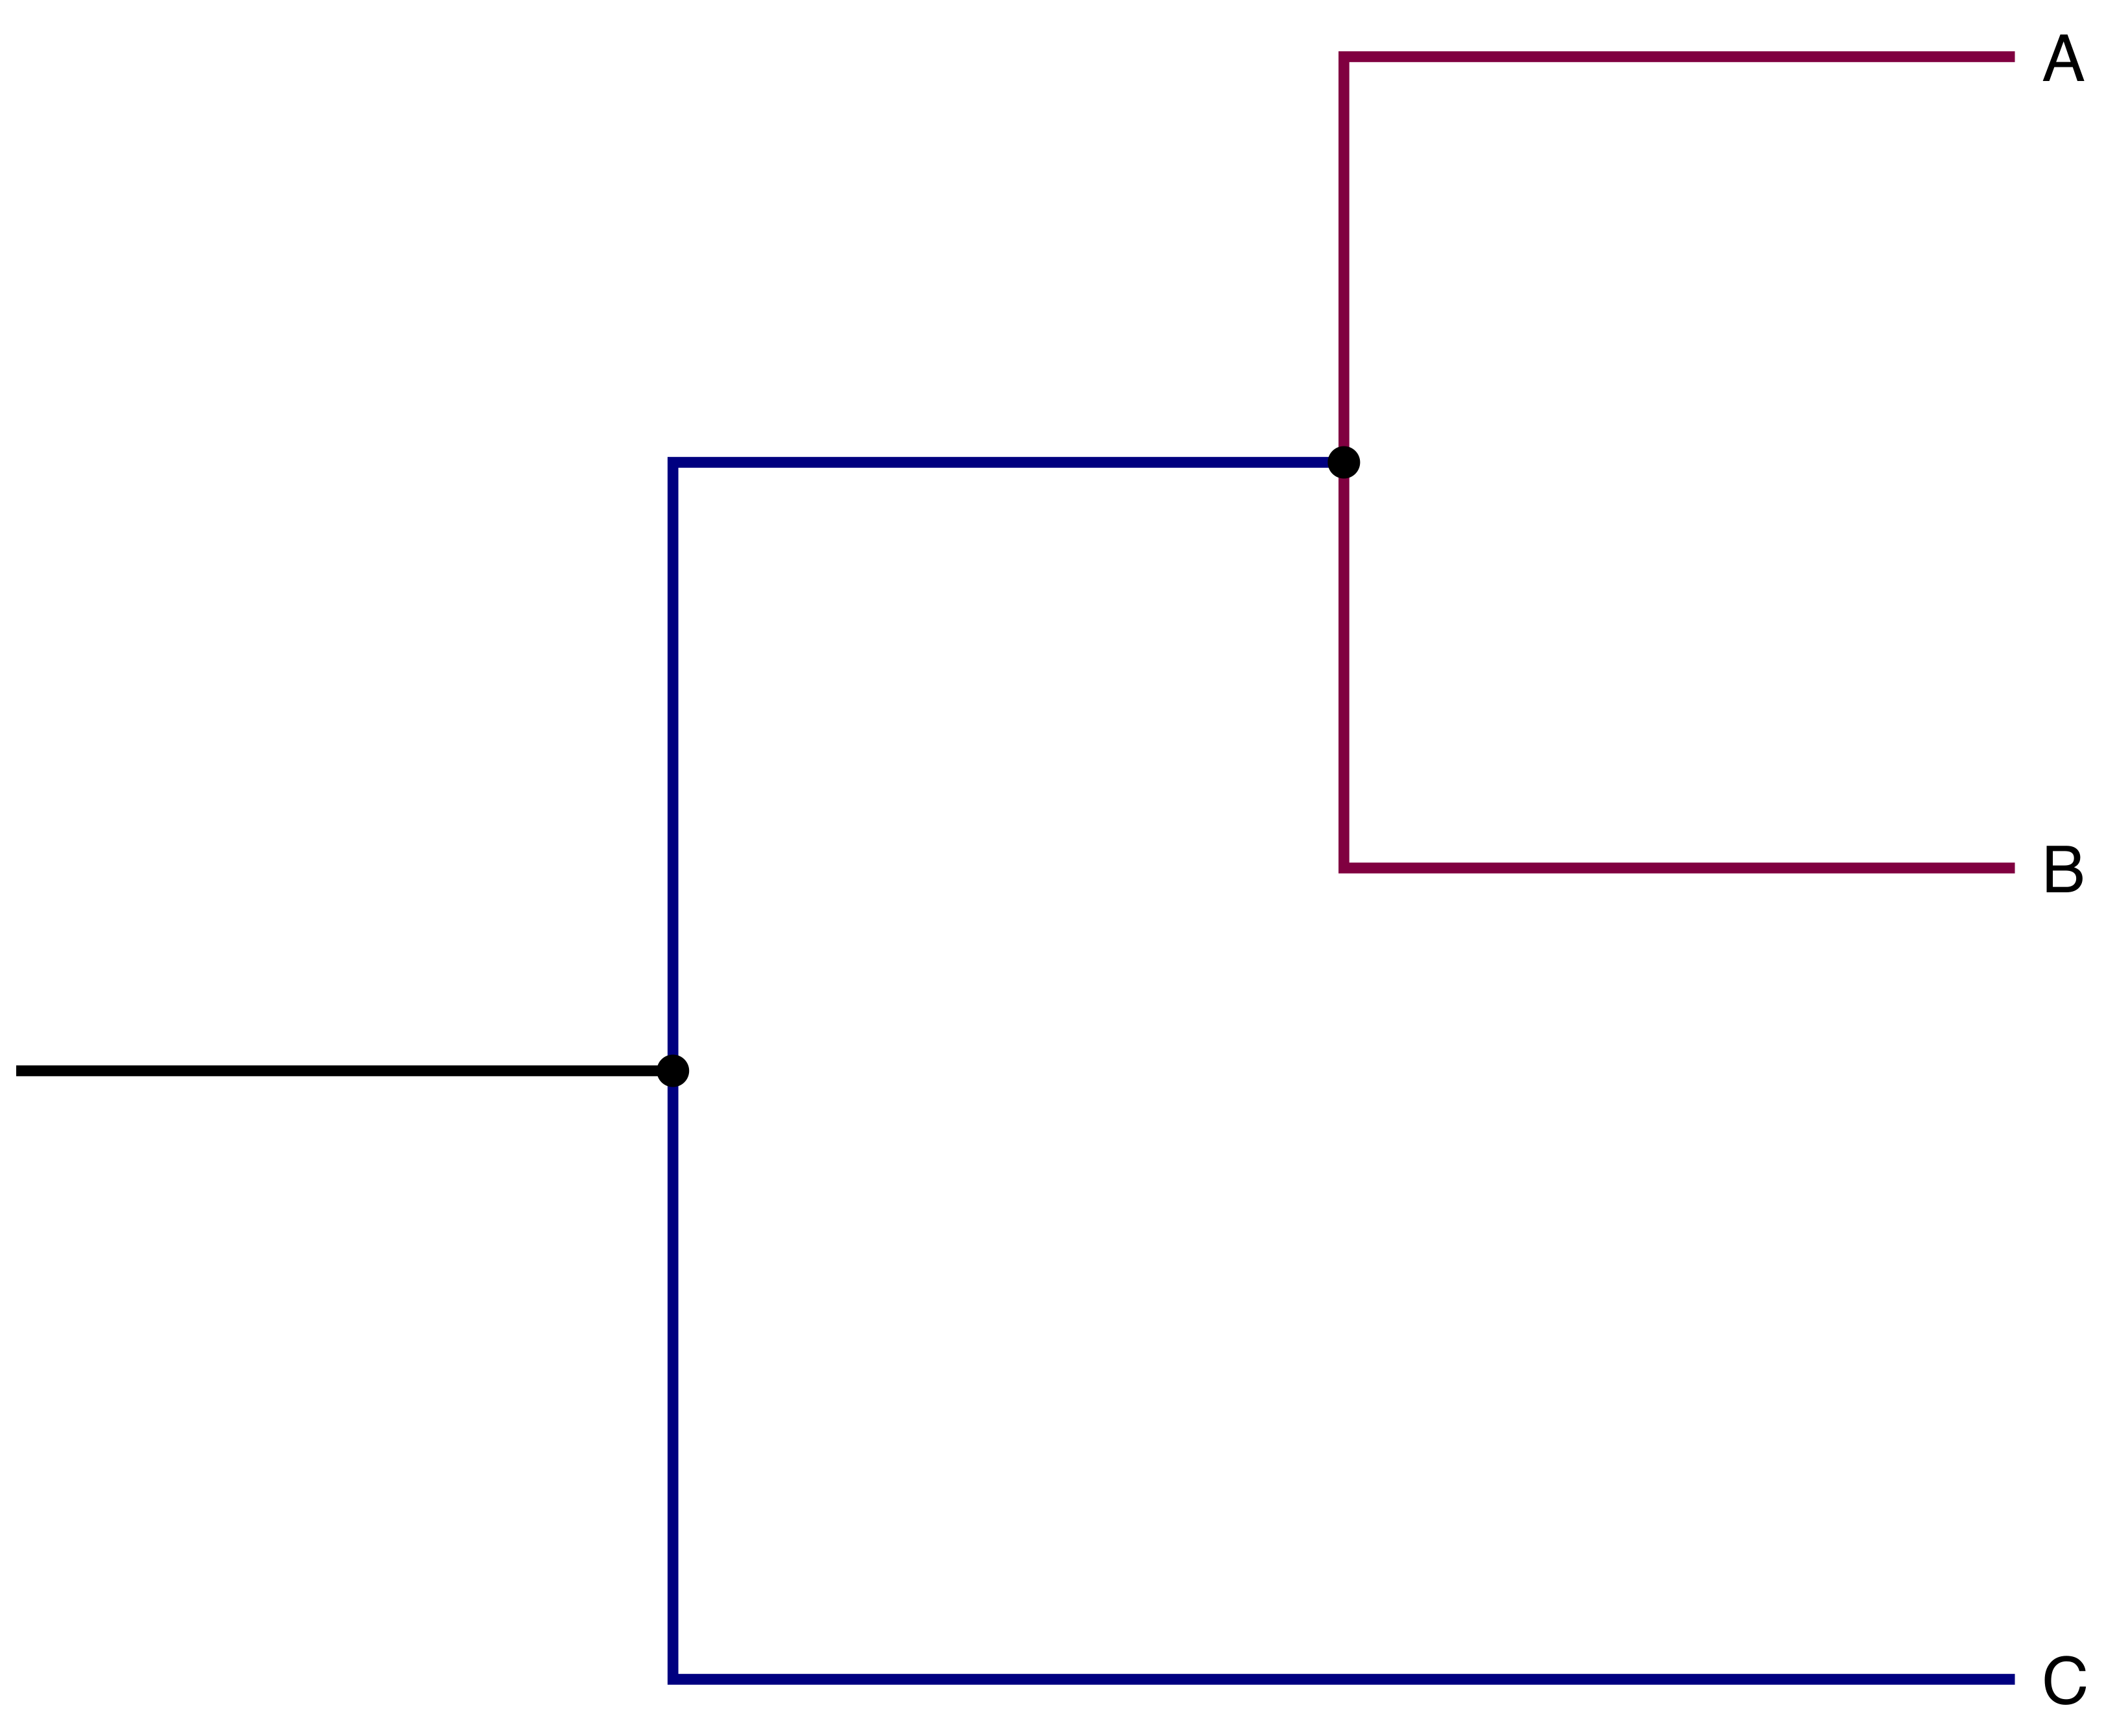
\includegraphics[width=0.5\linewidth]{{figures/phylo.png}}
\centering
\caption[Example of a population history]{
The relationships between populations A, B and C are depicted.
Note how branches of the same color can be simulated in parallel if there is no migration.
}
\label{fig:pop_hist}
\end{figure}

With tree sequences, it is possible to 
